\chapter{Non-Inverting Amplifier}
\section{Proof Of Concept}
\begin{figure}[tbp]
	\centering
	\begin{subfigure}{0.4\textwidth}
		\centering
		%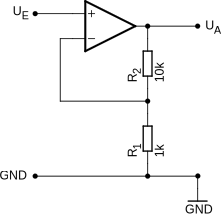
\includegraphics[width=.9\linewidth]{./img/schem-noninv.pdf}
		\caption{Basic Non-Inverting Amplifier with Gain 11}
		\label{schem:non_inv}
	\end{subfigure}
	\begin{subfigure}{0.4\textwidth}
		\centering
		%\includegraphics[width=.9\linewidth]{./img/non_inv_curve.pdf}
		\caption{Non-Inverting Amplifier:\newline $U_\text{pp,in}=\SI{55.2}{\milli\volt}, U_\text{pp,out}=\SI{600}{\milli\volt}$}
		\label{subfig:non_inv_curve}
	\end{subfigure}
	\caption{Schematic And Voltage Curves Of a Non-Inverting Setup}
\end{figure}
\autoref{schem:non_inv} shows the schematic of a non-inverting OpAmp.
As both inputs of the OpAmp virtually are at the same potential, the amplification can be calculated easily by using the voltage divider formula (as seen in \autoref{eq:bias_volt})
\begin{align*}
	U_\text{e}&=U_\text{a}\cdot\frac{R_1}{R_1+R_2} \\
	\Leftrightarrow\ A &=1+\frac{R_2}{R_1}.
\end{align*}
To examine the validity of this relation, the circuit is built and the output voltage is measured as a function of the input voltage.
The resulting curves are shown in \autoref{subfig:non_inv_curve}.
\begin{table}[tbp]
	\centering
	\caption{Input, output voltages $U_\text{pp,in/out}$ and resulting voltage amplification $A$ at $f=\SI{1}{\kilo\hertz}$}
	\label{tab:non_inv_vals}
	\begin{tabular}{SSS}
		\toprule
		{$U_\text{pp,in}$ in $\si{\milli\volt}$}&	{$U_\text{pp,out}$ in $\si{\volt}$}&	{$A$}\\
		\midrule
		\num{55.2}	&	\num{0.608}	&	\num{11.01}\\
		\num{352}	&	\num{3.96}	&	\num{11.25}\\
		\bottomrule
	\end{tabular}
\end{table}
In both measurements, the gain is $\approx 11$, which confirms the expectations.

\section{Input And Output Impedances}
\begin{figure}[tbp]
	\centering
	\begin{subfigure}{0.4\textwidth}
		\centering
		%\includegraphics[width=.9\linewidth]{./img/schem_shitty_circuit_1.pdf}
		\caption{Demonstrating High Input Impedance}
		\label{schem:shitty_circuit_1}
	\end{subfigure}
	\begin{subfigure}{0.4\textwidth}
		\centering
		%\includegraphics[width=.9\linewidth]{./img/schem_shitty_circuit_2.pdf}
		\caption{Demonstrating Low Output Impedance}
		\label{schem:shitty_circuit_2}
	\end{subfigure}
	\caption{Circuits For Demonstration Of I/O-Impedances}
\end{figure}
Lorem ipsum dolor sit amet, consectetur adipisicing elit, sed do eiusmod tempor incididunt ut labore et dolore magna aliqua. Ut enim ad minim veniam, quis nostrud exercitation ullamco laboris nisi ut aliquip ex ea commodo consequat. Duis aute irure dolor in reprehenderit in voluptate velit esse cillum dolore eu fugiat nulla pariatur. Excepteur sint occaecat cupidatat non proident, sunt in culpa qui officia deserunt mollit anim id est laborum.

\section{Frequency Response}
\begin{figure}[tbp]
	\centering
	\begin{subfigure}{0.4\textwidth}
		\centering
		\includegraphics[width=1.3\textwidth]{./data/plots/2_3.pdf}
		\caption{Amplification $A$ over Frequency $f$}
		\label{fig:noninvert_amp}
	\end{subfigure}
	\qquad\qquad
	\begin{subfigure}{0.4\textwidth}
		\centering
		\includegraphics[width=\textwidth]{./data/plots/2_3.pdf}
		\caption{Demonstrating Distortion At High Frequencies}
		\label{fig:noninvert_distortion}
	\end{subfigure}
\end{figure}

\autoref{fig:noninvert_amp} shows the frequency response curve of the non-inverting amplifier.
As expected, gain decreases with growing frequency, where the cutoff frequency roughly is $f_\text{cutoff}\approx\SI{61}{\kilo\hertz}$ ($\SI{-3}{\decibel}$).
\autoref{fig:noninvert_distortion} demonstrates that the output is distorted at high frequencies.
This behavior can be explained by an inertia of the OpAmp, which cannot \todo{regulate gate voltages, i know this is not exactly what happens but it's just physicists, feel free to reword} fast enough internally when frequencies are \todo{OVER 9000!}, so the output is delayed relative to the input and a square wave input signal effectively can be put out as a triangle signal, albeit the amplifier not being operated as an integrator.
